\section{Auswertung}
\label{sec:Auswertung}
\subsection{Die $γ$-Absorption}

Die Ungenauigeit der gemessenen Zerfälle bestimmt sich zu $\Delta Z = \sqrt{Z}$, da die Anzahl der Zerfälle
poissonverteilt sind.\\
Bei einer Nullmessung über 900s werden $Z_u = 567 \pm 24$ Zerfälle vom Zählrohr gemessen. Das entspricht einer
Impulsrate von 
\begin{align*}
  N_u = 0,63 \pm 0,03 \si{\per\second}.
\end{align*}
Die Ungenauigeit wurde mit der Gaußschen Fehlerfortpflanzung bestimmt.\\
Es werden nun verschieden dicke Eisen- und Bleiplatten zwischen Zählrohr und Strahler geschoben und Messungen 
durchgeführt. Die Ergebnisse lassen sich in \autoref{tab:1aFe} für Eisen und in \autoref{tab:1aPb} für Blei finden.\\
\begin{table}
  \centering
  \caption{Messergebnisse mit unterschiedlichen Eisenplatten.}
  \label{tab:1aFe}
  \begin{tabular}{c c c c}
    $d$ in \si{\milli\meter} & Messdauer $t$ in $\si{\second}$ & Anzahl Zerfälle $Z$  &  Impulsrate $N-N_u$ in $\si{\per\second}$\\
       \midrule
        $1,58 \pm 0,02$   &  300   &  $33377 \pm 183$ & $110,63 \pm 3,37$ \\
        $4,11 \pm 0,02$   &  300   &  $30768 \pm 175$ & $101,93 \pm 3,11$\\
        $6,50 \pm 0,02$   &  300   &  $27037 \pm 164$ & $89,49 \pm 2,74$\\
        $8,20 \pm 0,02$   &  300   &  $24383 \pm 156$ & $80,65 \pm 2,48$\\
        $10,92 \pm 0,02$  &  300   &  $21985 \pm 148$ & $72,65 \pm 2,24$\\
        $15,90 \pm 0,02$  &  300   &  $18337 \pm 135$ & $60,49 \pm 1,88$\\
        $18,20 \pm 0,02$  &  300   &  $15931 \pm 126$ & $52,47 \pm 1,64$\\
        $22,56 \pm 0,02$  &  300   &  $10510 \pm 103$ & $34,40 \pm 1,11$\\
        $39,81 \pm 0,02$  &  300   &  $ 6657 \pm 82$ & $21,56 \pm 0,74$\\
        $50,00 \pm 0,02$  &  300   &  $ 4557 \pm 68$ & $14,56 \pm 0,54$\\
      \bottomrule
    \end{tabular}
\end{table}

\begin{table}
  \centering
  \caption{Messergebnisse mit unterschiedlichen Bleiplatten.}
  \label{tab:1aPb}
  \begin{tabular}{c c c c}
    $d$ in \si{\milli\meter} & Messdauer $t$ in $\si{\second}$ & Anzahl Zerfälle $Z$  &  korrigierte Impulsrate $N-N_u$ in $\si{\per\second}$\\
       \midrule
        $3,79 \pm 0,02$   &  300   &  $24245 \pm 156$ & $80,19 \pm 2,47$ \\
        $5,20 \pm 0,02$   &  300   &  $22575 \pm 150$ & $74,52 \pm 2,29$\\
        $9,40 \pm 0,02$   &  200   &  $11221 \pm 106$ & $55,48 \pm 1,74$\\
        $14,30 \pm 0,02$  &  200   &  $5936  \pm 77$ & $29,05 \pm 0,97$\\
        $20,00 \pm 0,02$  &  200   &  $3926  \pm 63$ & $19,00 \pm 0,69$\\
        $26,18 \pm 0,02$  &  200   &  $2067  \pm 45$ & $9,71 \pm 0,43$\\
        $46,10 \pm 0,02$  &  200   &  $602   \pm 25$ & $0,37 \pm 0,24$\\
      \bottomrule
    \end{tabular}
\end{table}

Es werden für Eisen zehn verschiedene Dicken an Platten verwendet, bei Blei sieben. Es werden zudem 
die um den Nulleffekt korrigierten Impulsraten $N-N_u$ berechnet und eingetragen.\\
Nachfolgend werden die Absorptionskoeffizienten $ \mu $ bestimmt. Dazu wird \autoref{eqn:Absorptionsgesetz}
verwendet. Der Logarithmus der korrigierten Impulsraten wird gegen die Schichtdicke $d$ aufgetragen, wodurch sich
ein linearer Zusammnehang ergibt. Die lineare Regression der Form $f(x) = mx +b$ liefert für die Geraden folgende Werte:
\begin{align*}
  m_{Fe} = -42,7 \pm 2,0 \\
  b_{Fe} = 4,7 \pm 0,1 \\
  m_{Pb} = -85,6 \pm 3,5 \\
  b_{Pb} = 4,7 \pm 0,1 \\
\end{align*}

Die Fehlerfortpflanzung wurde mittels dem Python package uncertainties bestimmt. \cite{unc}

\begin{figure}
  \centering
  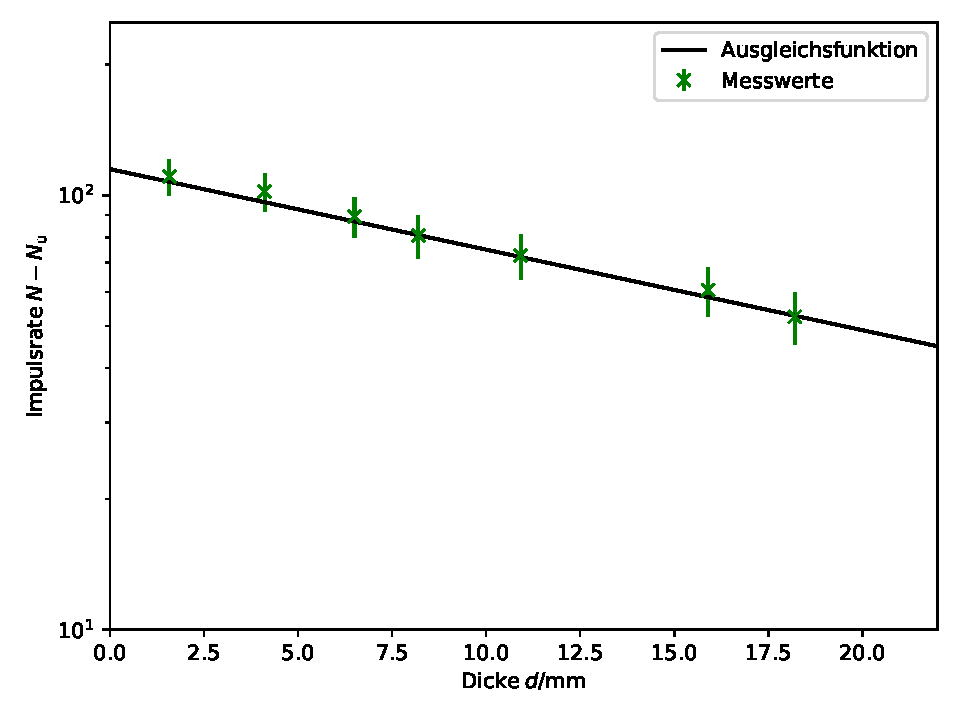
\includegraphics{Bilder/Eisen.pdf}
  \caption{Logarithmus der korrigierten Impulsrate bei Eisen aufgetragen gegen die Schichtdicke $d$}
  \label{fig:Eisen}
\end{figure}
\begin{figure}
  \centering
  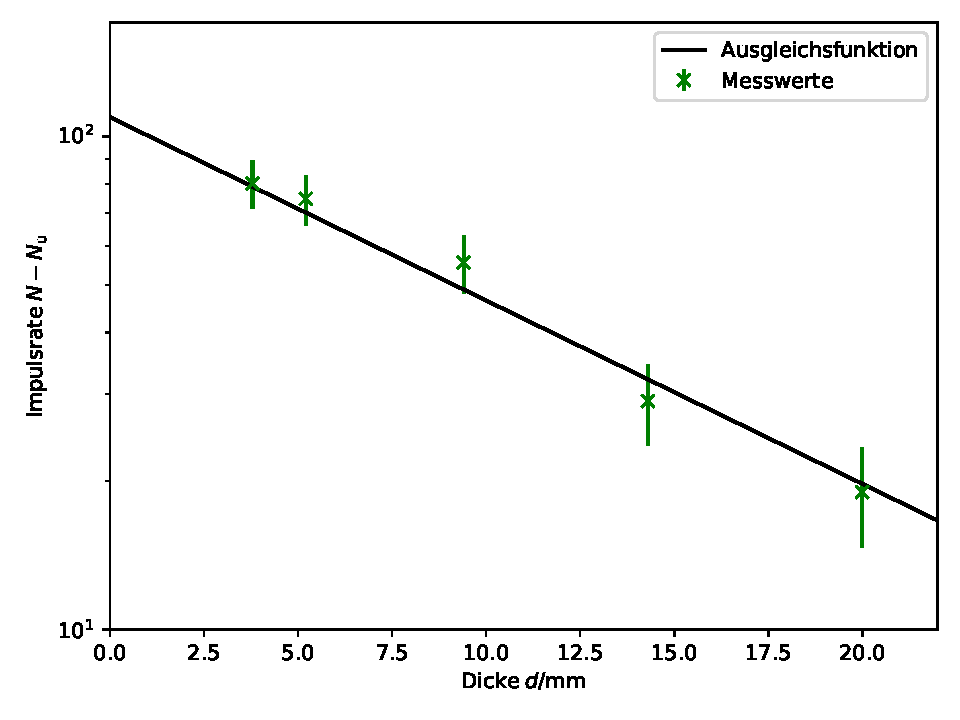
\includegraphics{Bilder/Blei.pdf}
  \caption{Logarithmus der korrigierten Impulsrate bei Blei aufgetragen gegen die Schichtdicke $d$}
  \label{fig:Blei}
\end{figure}

Durch die Geradensteigungen und y-Achsenabschnitte der Geraden in \autoref{fig:Eisen} und \autoref{fig:Blei} 
lassen sich nun nach \autoref{eqn:Absorptionsgesetz} die Absorptionskoeffizienten $\mu_{Fe}$ und $\mu_{Pb}$ 
bestimmen, sowie $N_0$ der beiden Materialien:\\
\begin{align*}
  \mu_{Fe} &= (42,7 \pm 2,0) \, \si{\per\meter} \\
  N_{0,Fe} &= (110 \pm 1) \, \si{\per\second} \\
  \mu_{Pb} &= (85,6 \pm 3,5) \, \si{\per\meter} \\
  N_{0,Pb} &= (110 \pm 1) \, \si{\per\second} \\
\end{align*}

Die Fehlerfortpflanzungen der Gleichungen wurden erneut allesamt mittels dem Python package 
uncertainties bestimmt. \cite{unc}

\subsection{Vergleich mit den aus der Theorie berechneten Absorptionskoeffizienten}

Um Schlüsse über die vorliegenden Absorbtionsmechanismen zu ziehen, werden die gemessenen Absorptionskoeffizienten
mit gerechneten Werten verglichen. Die Absorptionskoeffizienten $\mu_{Com}$ werden durch \autoref{eq:sigma_c} und
\autoref{eq:mu_c} berechnet.
Für diese Gleichungen werden einige Materialkonstanten benötigt, diese werden in \autoref{tab:Material} notiert.
\begin{table}
  \centering
  \begin{tabular}{S S[table-format=2.0] S[table-format=3.1] S[table-format=2.3]}
    \toprule
    {Material} & {Ordnungszahl $Z$} & {Masse $m\:$ in $\frac{\si\gram}{\si\mol}$} & {Dichte $\rho\:$ in $\frac{\si\gram}{\si{\centi\meter}^3}$}\\
    \midrule
    \text{Blei} & 82 & 207.2 & 11.342\\
    \text{Eisen} &26 & 55.8  & 7.874\\
    \bottomrule
  \end{tabular}
  \caption{Materialkonstanten von Eisen und Blei zur Bestimmung des Absorbtionskoeffizienten.}
  \label{tab:Material}
\end{table}
Es wird zudem die charakteristische Größe $\epsilon = 1,295$ für Caesium verwendet.
Einsetzen ergibt nun:
\begin{equation*}
  \sigma_{Com} = 2,57 \cdot 10^{-29} \, \mathrm{m}^2
\end{equation*}
und dadurch die Absorbtionskoeffizienten
\begin{align*}
  \mu_{Com,Fe} = 56,76 \, \si{\per\meter} \, \mathrm{und} \\
  \mu_{Com,Pb} = 69,43 \, \si{\per\meter}. \\
\end{align*}

\subsection{\texorpdfstring{$\beta^-$}{Beta}-Absorption}

Um die Maximalenergie von $^{99}$Tc zu bestimmen, wird mithilfe der aufgenommenen Messwerte eine
$\beta$-Absorptionskurve erstellt.\\
In \autoref{tab:Aluminium} sind die Messwerte zu verschiedenen Dicken der Aluminiumplatten eingetragen,
sowie die berechneten korrigierten Impulsraten $N - N_u$.
\begin{table}
  \centering
  \caption{Messergebnisse mit unterschiedlichen Aluminiumplatten.}
  \label{tab:Aluminium}
  \begin{tabular}{c c c c}
    $d$ in \si{\micro\meter} & Messdauer $t$ in $\si{\second}$ & Anzahl Zerfälle $Z$  &  korrigierte Impulsrate $N-N_u$ in $\si{\per\second}$\\
       \midrule
       $100 \pm 0,5$ &    500  &   $14164 \pm 119$  & $27,70 \pm 0,86$ \\
       $125 \pm 1$ &   500   &   $3514 \pm 59$  &     $6,40 \pm 0,22$\\
       $153 \pm 1$  & 600   &   $4317 \pm 66$ &       $6,57 \pm 0,23$\\
       $160 \pm 1$  &  600  &    $2595 \pm 51$  &     $3,70 \pm 0,14$\\
       $200 \pm 1$  & 700    &  $1199 \pm 35$ &       $1,08 \pm 0,06$\\
       $253 \pm 1$  &  700   &    $523 \pm 23$  &     $0,12 \pm 0,03$\\
       $302 \pm 1$  & 700    &  $ 506 \pm 22$ &       $0,09 \pm 0,03$\\
       $400 \pm 1$  & 700   &    $466 \pm 22$ &       $0,04 \pm 0,03$\\
       $482 \pm 1$  &  700  &    $ 495 \pm 20$  &     $0,08 \pm 0,03$\\
      \bottomrule
    \end{tabular}
\end{table}
Die korrigierte Impulsrate wird nun logarithmisch gegen die Schichtdicke $d$ aufgetragen, wodurch die
Massenbelegung $R_{max}$ und die Gesamtenergie $E_{max}$ berechnet werden können. Die maximale Reichweite
ist der Schnittpunkt zwischen der Ausgleichsgeraden des vorderen Bereichs der Messwerte und der Ausgleichsgeraden
des hinteren Bereichs der Messwerte.\\
Die lineare Regression der Form $f(x) =mx+b$ ergibt folgende Werte:
\begin{align*}
  m_1 = -29710 \pm 5011 \\
  b_1 = 6.1 \pm 0.8 \\
  m_2 = -2.6 \pm 0.3 \\
  b_2 = 0 \\
\end{align*}
Dadurch ergibt sich die maximale Reichweite $D = 0,000292 \pm 0,000056$ m. Mit der Massenbelegung $R_{max} = \rho D$ lässt
sich dann mit \autoref{eqn:emax} die Gesamtenergie bestimmen zu $E_{max} = (0,295 \pm 0,115)$ MeV.
\begin{figure}
  \centering
  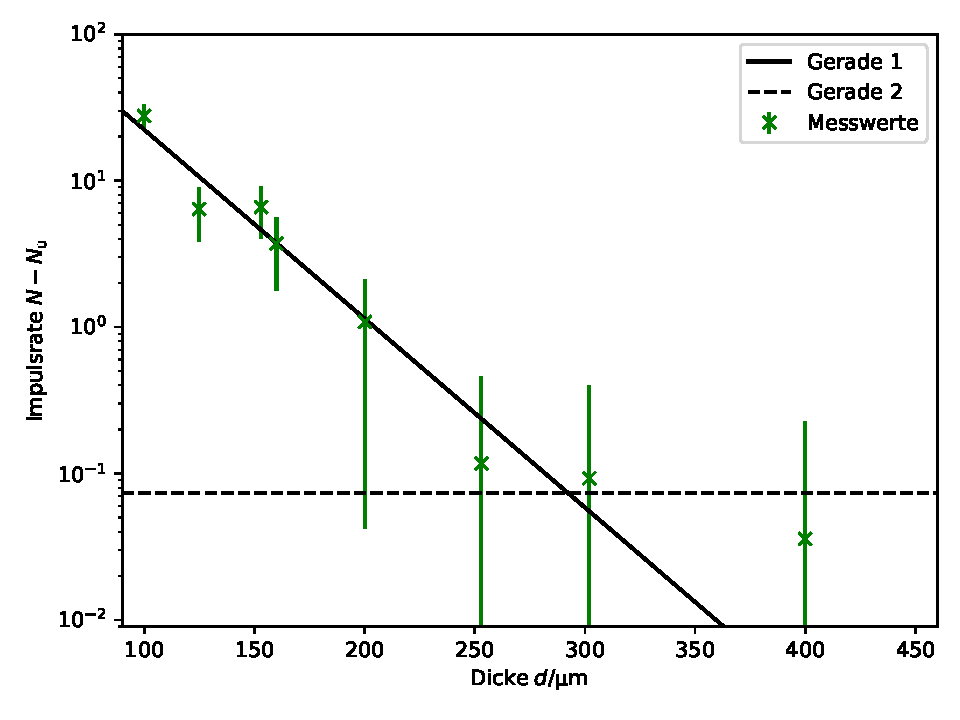
\includegraphics{Bilder/beta.pdf}
  \caption{Logarithmus der korrigierten Impulsrate bei Alluminium aufgetragen gegen die Schichtdicke $d$}
  \label{fig:Beta}
\end{figure}